% 2011 年江苏卷第 17 题：正方形硬纸片折叠成正四棱柱包装盒。
% 来源 PDF：普通高考/2011/2011江苏.pdf，SHA-256 71763ef5d0c2b5800c12515e6b3addb77e585b2460fd11c1013fcec6f050ece9。
% 原页：第 1 页第 3 栏上部，书页码 675。示意图，不按比例。
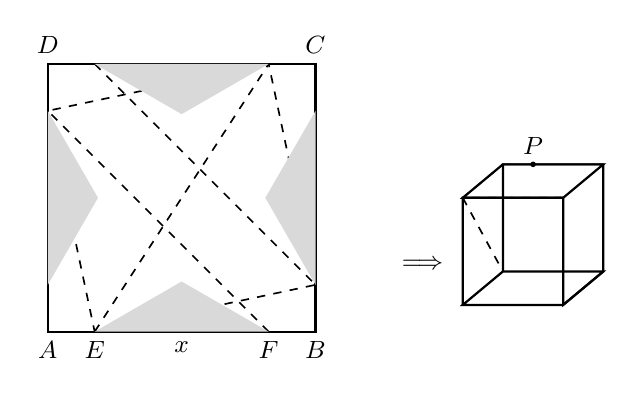
\begin{tikzpicture}[>=stealth, semithick, font=\small, scale=0.85]
  % 左：正方形纸片
  \coordinate (A) at (0,0);
  \coordinate (B) at (4,0);
  \coordinate (C) at (4,4);
  \coordinate (D) at (0,4);
  \coordinate (E) at (0.7,0);
  \coordinate (F) at (3.3,0);
  \coordinate (G) at (4,0.7);
  \coordinate (H) at (3.3,4);
  \coordinate (I) at (0,3.3);
  \coordinate (J) at (0.7,4);
  \draw[thick] (A)--(B)--(C)--(D)--cycle;
  % 折痕
  \draw[dashed] (E)--(G)--(H)--(I)--cycle;
  \draw[dashed] (E)--(H);
  \draw[dashed] (F)--(I);
  \draw[dashed] (J)--(G);
  % 切去的四个等腰直角三角形
  \fill[gray!30] (E)--(F)--(2,0.75)--cycle;
  \fill[gray!30] (J)--(H)--(2,3.25)--cycle;
  \fill[gray!30] (I)--(0.75,2)--(0,0.7)--cycle;
  \fill[gray!30] (G)--(4,3.3)--(3.25,2)--cycle;
  \node[below] at (A) {$A$};
  \node[below] at (B) {$B$};
  \node[above] at (C) {$C$};
  \node[above] at (D) {$D$};
  \node[below] at (E) {$E$};
  \node[below] at (F) {$F$};
  \node[below] at (2,0) {$x$};
  % 右：折成的正四棱柱
  \begin{scope}[xshift=6.2cm, yshift=0.4cm]
    \coordinate (a) at (0,0); \coordinate (b) at (1.5,0);
    \coordinate (c) at (2.1,0.5); \coordinate (d) at (0.6,0.5);
    \coordinate (a1) at (0,1.6); \coordinate (b1) at (1.5,1.6);
    \coordinate (c1) at (2.1,2.1); \coordinate (d1) at (0.6,2.1);
    \draw[thick] (a)--(b)--(c)--(d)--cycle;
    \draw[thick] (a)--(a1)--(b1)--(b)--(c)--(c1)--(d1)--(d);
    \draw[thick] (a1)--(b1)--(c1)--(d1)--cycle;
    \draw[dashed] (d1)--(d);
    \draw[dashed] (a1)--(d);
    \draw[dashed] (b1)--(a1) -- (d1);
    \fill (1.05,2.1) circle (1.2pt) node[above] {$P$};
  \end{scope}
  \node at (5.6,1.0) {$\Longrightarrow$};
\end{tikzpicture}
